\section{Resultat}
I avsnitt \ref{avsnitt:fragestallning} framfördes frågeställningarna:

\begin{enumerate}
\item Vilket av de två byggsystemen har bäst prestanda?
\item Vilket byggsystem är lättast att använda och utveckla?
\item Hur hade projektet påverkats av ett annat val av byggsystem?
\end{enumerate}

\noindent Efter undersökningen beskriven i avsnitt \ref{avsnitt:metod} kan svaren på dessa frågor ges här.

\subsection{Prestanda}
Resultatet från prestandamätningarna syns i tabell \ref{tabell:prestanda} och i figur \ref{fig:prestanda}.

\begin{table}[h!]
  \centering
  \begin{tabular}{|l|l|l|}
    \hline
    \textbf{Trådar} & \textbf{Make} (s) & \textbf{SCons} (s) \\ \hline
    1 & 2.65 & 3.62 \\ \hline
    2 & 1.56 & 2.34 \\ \hline
    4 & 1.32 & 2.19 \\ \hline
    8 & 1.32 & 2.20 \\ \hline
    16 & 1.34 & 2.25 \\ \hline
  \end{tabular}
  \caption{Resultat från prestandatester.}
  \label{tabell:prestanda}
\end{table}

\begin{figure}[h!]
  \centering
  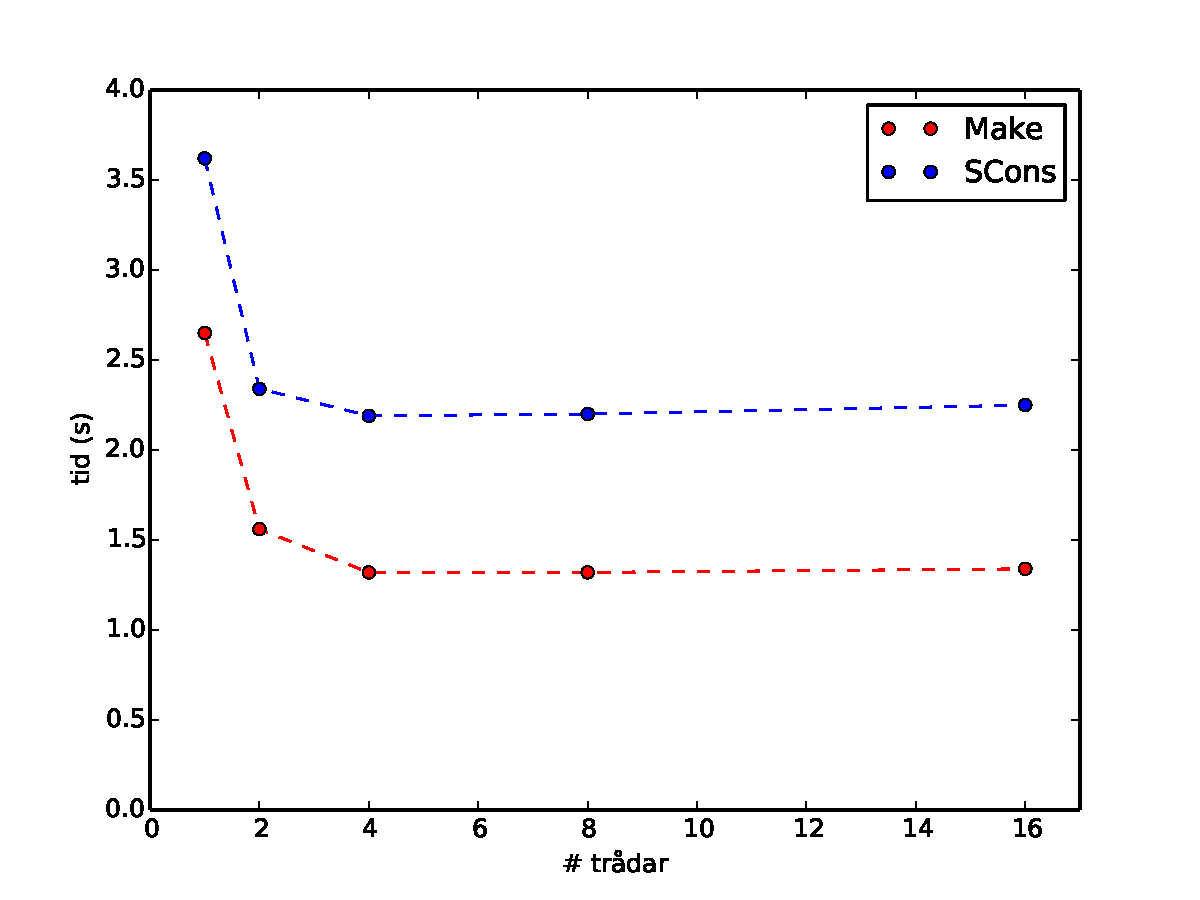
\includegraphics[scale=0.6]{yngve-tex/grafik/prestanda.pdf}
  \caption{Resultat från prestandatester.}
  \label{fig:prestanda}
\end{figure}

\FloatBarrier

\subsection{Användning och vidareutveckling}
Kandidatgruppen framförde ett flertal synpunkter som sammanfattas i följande lista:

\begin{itemize}
  \item Användningen är densamma, bara olika kommandon.
  \item Alla känner till Make, ingen visste om SCons sen innan.
  \item SCons-filerna är mer lättförståeliga än Makefilerna.
  \item Det var enkelt att sätta sig in i SCons då det är vanlig Pythonkod.
  \item Makes deklarativa stil såg främmande och spännande ut.
\end{itemize}

\subsection{Byggsystemets påverkan på projektet}
Då prestandaskillnaden för ett projekt av den här storleken är så pass liten så påverkar valet av byggsystem inte utvecklarens dagliga arbetsrutiner nämnvärt. Det som påverkas är istället möjligheten till underhåll och vidareutveckling av byggsystemet i takt med att projektet växer. 
